
%\section{OASys--based Engineering Methodology Applied to RCT}

The \emph{ASys Engineering Methodology} developed in ICEA is based on the OASys ontology and has been applied to the Robot Control Testbed for its conceptual analysis. The following sections provide a description on how the different tasks were accomplished, with examples of the different workproducts obtained. The terms in italic that appear in the phases, tasks, subtasks and models descriptions are those defined in the Packages of OASys.\\

\section{RCT ASys Views Phase}
The purpose of this \emph{Phase} is to identify the different views of interest for the RCT considering the Perspective Package elements, specialised through the ASysPerspective Package concepts. \\

For example the \emph{RequirementViewpoint} especilises the concept of \emph{Viewpoint} to address the analysis of the RCT from a \emph{ASysRequirement} \emph{Concern}, to establish the different requirements to be defined in the system. Considering this viewpoint, a RCTRequirementViewpointModel can be instantiated (Fig. \ref{fig:RCTrequirementviewpointmodel}). The different concepts, relationships and attributes where chosen from the Perspective and the ASysPerspective Package. The original concepts have been ontologically instantiated into RCT related ones. For example, the concept RCTRequirement is an \emph{ASysRequirement} concern, which in turn is a\emph{Concern} from the Perspective Package. In a similar way, RCTPerformanceViewpoint is a \emph{Viewpoint}, as defined in the Perspective Package. \\

\begin{figure}[htbp]
\begin{center}
 {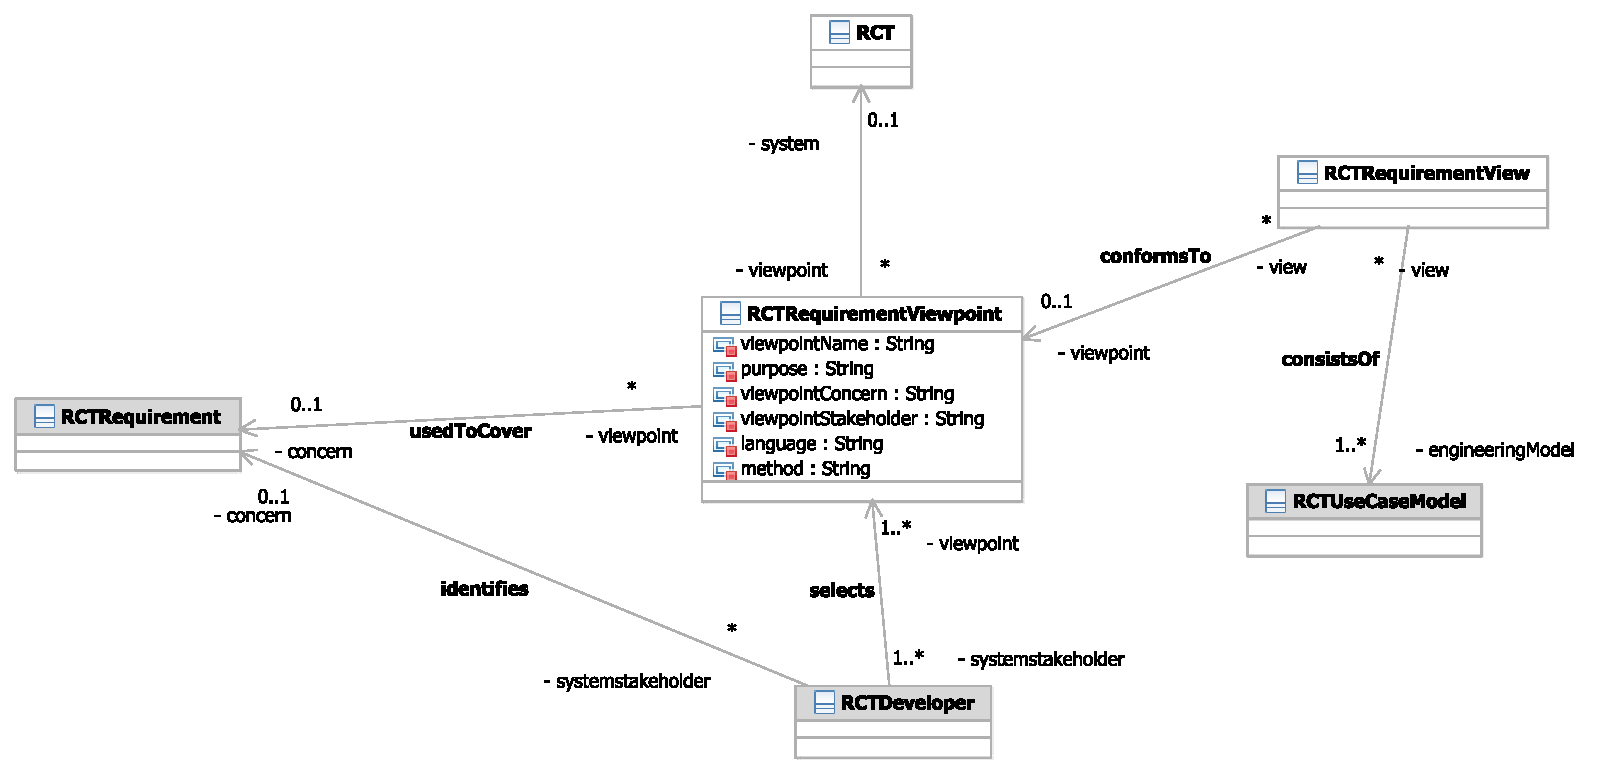
\includegraphics[width=0.95\textwidth]{RCT_RCTRequirementViewpointModel.pdf}}
\end{center}
\caption{RCT RequirementViewpoint Model}
\label{fig:RCTrequirementviewpointmodel}
\end{figure}

The \emph{StructuralViewpoint} pays attention to the au- 
tonomous system structure, as considering the \emph{ASysStructure} concern. A RCTStructuralViewpointModel can be obtained (Fig. \ref{fig:RCTrequirementviewpointmodel}) by instantiating the different concepts, relationships and attributes in the Perspective and the ASysPerspective Packages. In this model,  the RCTStructuralView is a \emph{View} that will consist of a RCTStructuralModel, which is the \emph{EngineeringModel} to be obtained as output of the StructuralAnalysis task.\\

\begin{figure}[htbp]
\begin{center}
 {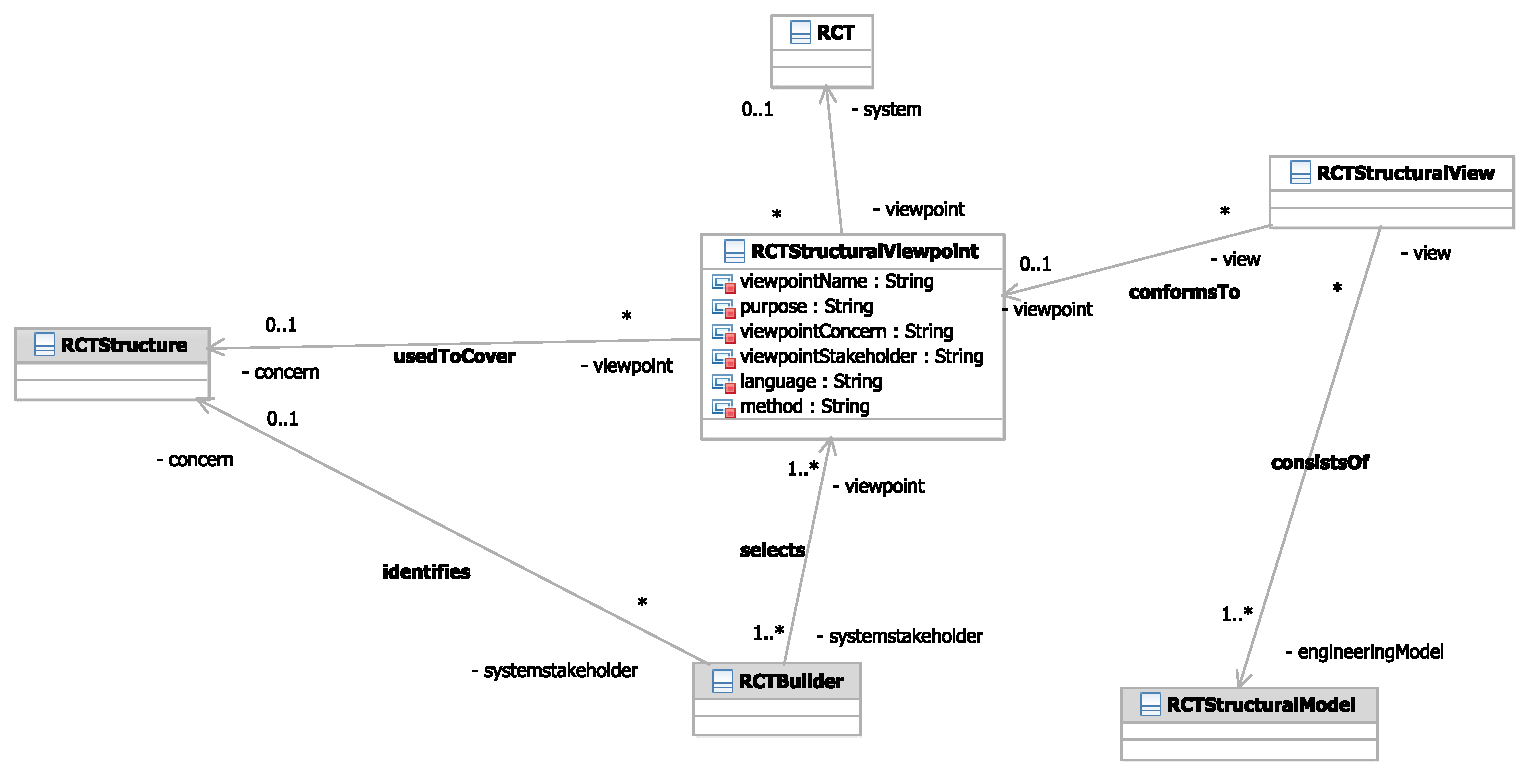
\includegraphics[width=0.95\textwidth]{RCT_RCTStructuralViewpointModel.pdf}}
\end{center}
\caption{RCT StructuralViewpoint Model}
\label{fig:RCTstructuralviewpointmodel}
\end{figure}

Additionally, the \emph{BehaviouralViewpoint} describes the autonomous system's behaviours, i.e., how the system operates under certain conditions. The RCTBehaviouralViewpointModel obtained (Fig. \ref{fig:RCTbehaviouralviewpointmodel}) instantiates the concepts and relationships in the Perspective and the ASysPerspective Packages. The different roles played for the concepts in the model are shown in each one of the relationships, which are given the same name as in the original package.\\


\begin{figure}[htbp]
\begin{center}
 {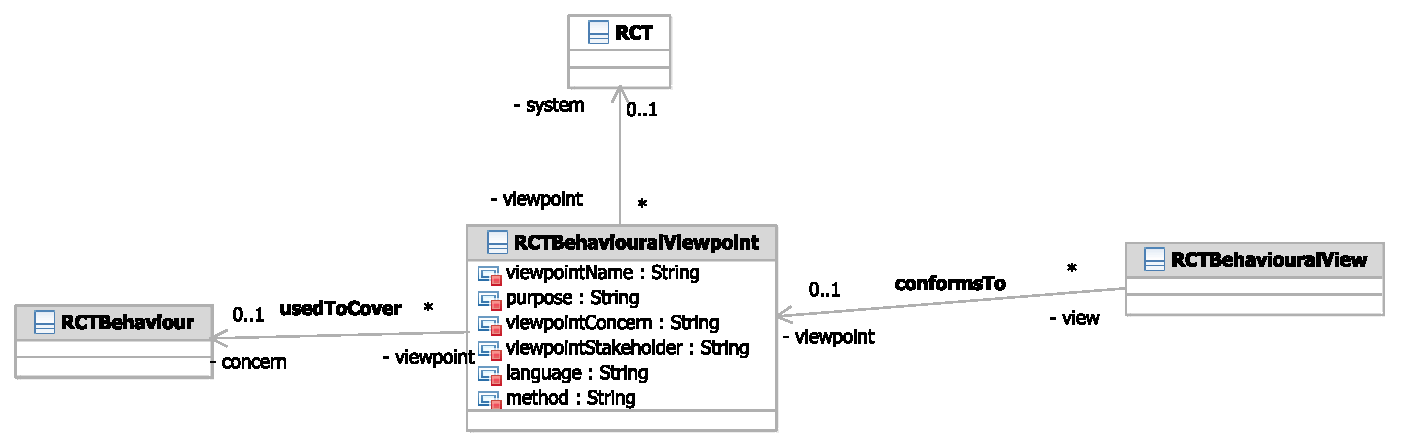
\includegraphics[width=0.95\textwidth]{RCT_RCTBehaviouralViewpointModel.pdf}}
\end{center}
\caption{RCT BehaviouralViewpoint Model}
\label{fig:RCTbehaviouralviewpointmodel}
\end{figure}

In turn, the \emph{FunctionalViewpoint} focus on the analysis of an autonomous system's functions, as desired or expected behaviours. The RCTStructuralViewpointModel (Fig. \ref{fig:RCTfunctionalviewpointmodel}) instantiates the  Perspective and the ASysPerspective Packages ontological elements, focusing on the functional aspects to consider for the RCT. In this model,  the RCTFunctionalView is a \emph{View} formalises as a RCTFunctionalModel, which is the \emph{EngineeringModel} consisting of different function related models, obtained as outputs of the FunctionalModelling subtask.\\

\begin{figure}[htbp]
\begin{center}
 {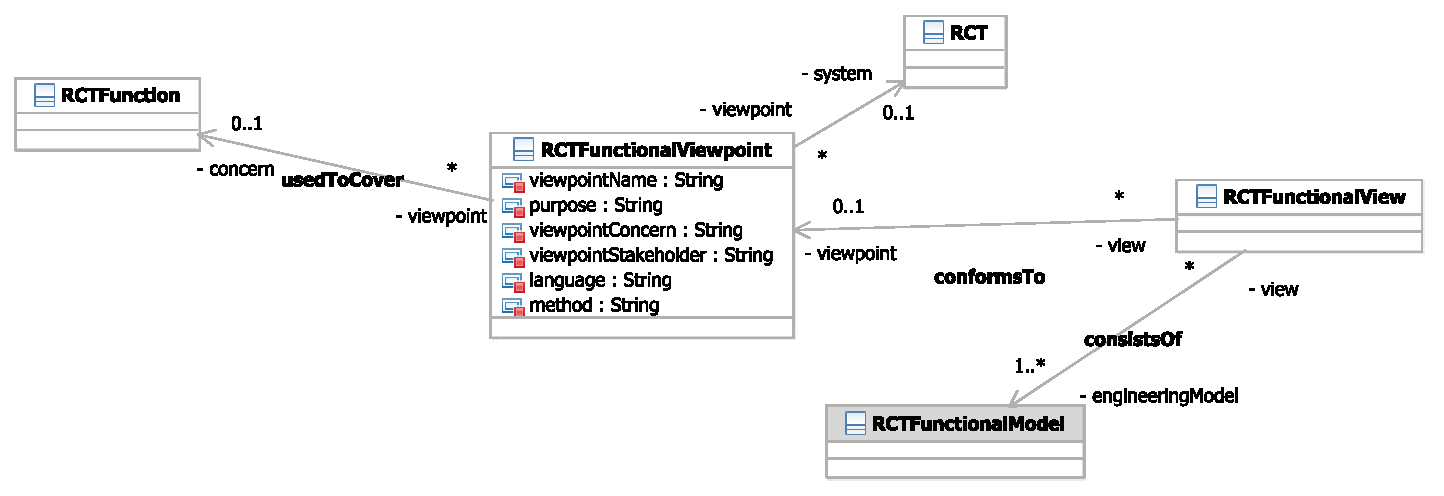
\includegraphics[width=0.95\textwidth]{RCT_RCTFunctionalViewpointModel.pdf}}
\end{center}
\caption{RCT FunctionalViewpoint Model}
\label{fig:RCTfunctionalviewpointmodel}
\end{figure}



During the RCT development, it will be necessary to address the \emph{PerformanceViewpoint}, to evaluate the performance requirements and benchmarking of the RCT once it is finally implemented. The PerformanceViewpoint addresses the performance aspects of the RCT. The Perspective and the ASysPerspective Package ontological elements were used to build up a PerformanceViewpointModel for the RCT (Fig. \ref{fig:RCTperformanceviewpointmodel}).\\

\begin{figure}[htbp]
\begin{center}
 {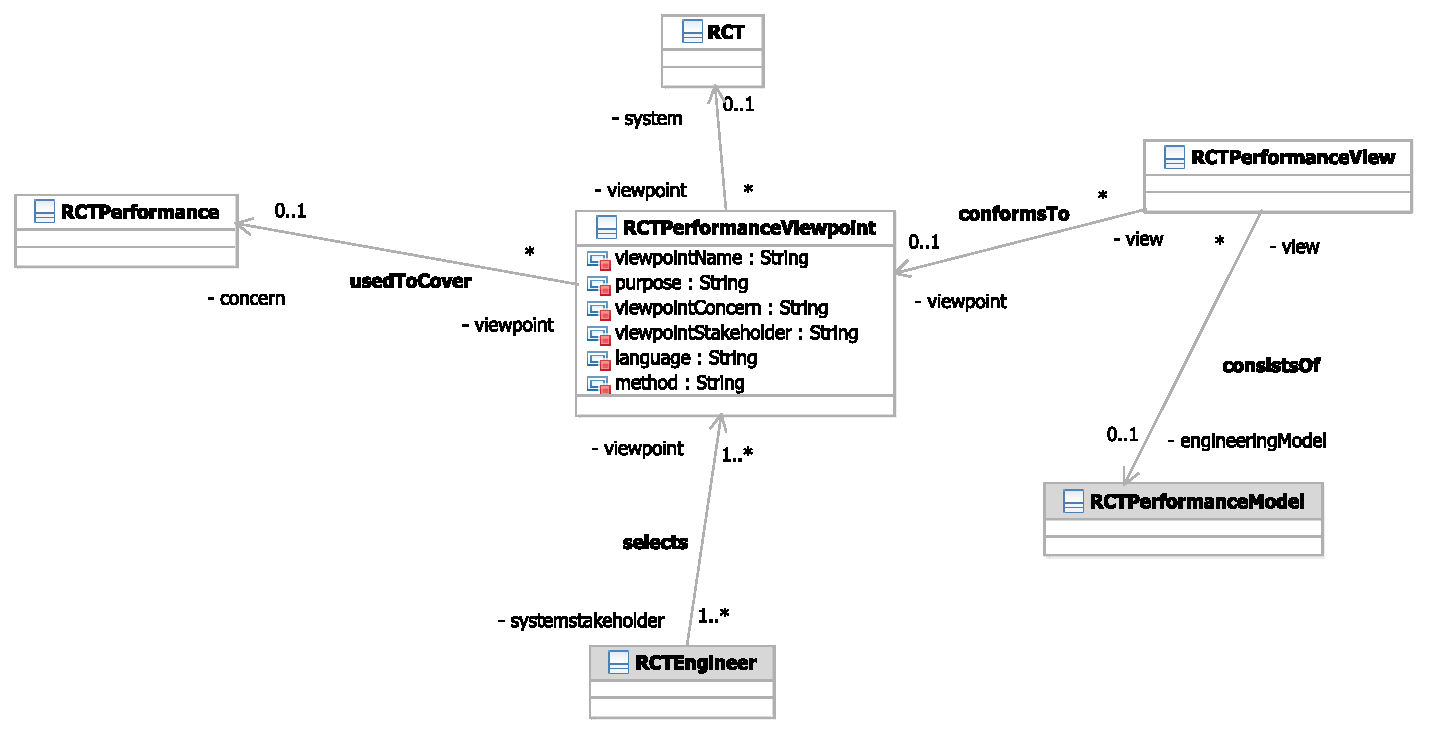
\includegraphics[width=0.95\textwidth]{RCT_RCTPerformanceViewpointModel.pdf}}
\end{center}
\caption{RCT PerformanceViewpoint Model}
\label{fig:RCTperformanceviewpointmodel}
\end{figure}


\section{RCT ASys Requirement Phase}

The purpose of this phase is to identify and elicit stakeholders' requirements for the RCT considering the RequirementViewpoint. The requirements are to be specified during this phase, by using traditional requirements engineering techniques.\\ 

\begin{itemize}
\item System UseCase Task

The first \emph{Task} during the \emph{ASys Requirement Phase} is to analyse the \emph{System UseCase}s, by instantiating the Requirement Package' ontological elements in the SystemEngineering Subontology. This \emph{Task} consists of the \emph{Subtask}s of \emph{UseCaseModelling} and \emph{UseCaseDetailing}, as defined in the ASys Engineering Subontology.\\

An \emph{UseCase} in OASys has been defined as a mean to capture a requirement of a system, as defined in the Perspective Package.To define the UseCase, the \emph{Subject} as system under consideration, and the different \emph{UseCaseActor}s as objects that interact with the system are also identified, among other aspects. As a result, a \emph{SystemUseCaseModel} is obtained, detailing the previous identified elements. The UML classes in the model are instantiation of the original OASys concepts, this fact being specified by the UML roles names in the shown associations. \\




When the \emph{Subject} under study is the Robot Control Testbed, an RCT \emph{UseCaseModel} shows the RCT's requirements by means of use cases. A system's requirements can be of different types (physical, functional, performance, interface, design) as defined in the Requirement Package.  An initial requirement analysis made by the RCT developers, identified the \emph{FunctionalRequirement}s for the RCT, where this concept has been defined as a ''requirement that specifies an operation or behaviour that a system must perform'' in OASys. Primary \emph{FunctionalRequirement}s for the RCT are to navigate, as well as to survive.\\

The navigation requirement is captured by means of the \emph{UseCase} Navigation, which \emph{include}s the secondary \emph{FunctionalRequirement}s of being able to explore the environment, identify elements in the environment, and to avoid obstacles. These requirements are captured in the \emph{Usecase}s of EnvironmentExploration, Identification and ObstacleAvoidance respectively (Fig. \ref{navigationusecasemodel}). In turn, the \emph{FunctionalRequirement} of surviving is captured in the Survival \emph{UseCase}, which \emph{include}s the SubsystemFailure and Recharge \emph{UseCase}s (Fig. \ref{survivalusecasemodel}).  \\

\begin{figure}[htbp]
\begin{center}
 {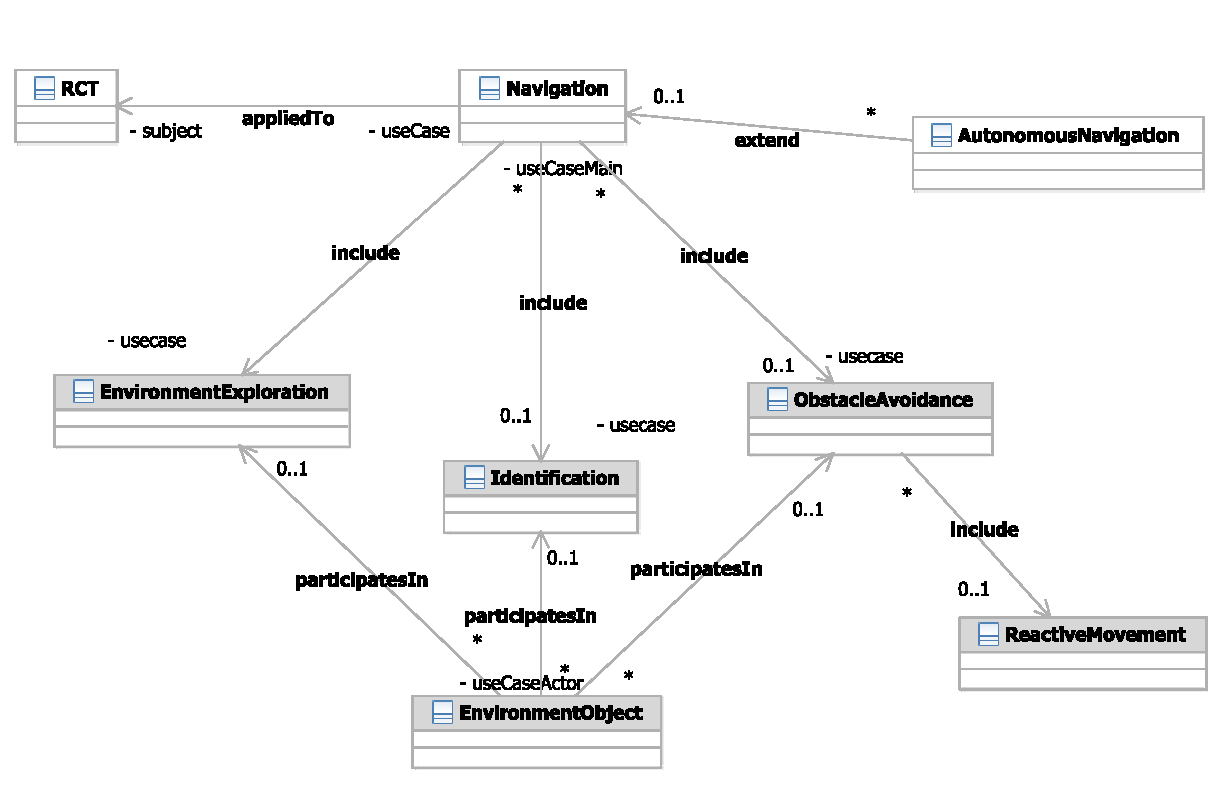
\includegraphics[width=0.95\textwidth]{RCT_RCTNavigationUseCaseModel.pdf}}
\end{center}
\caption{RCT Navigation UseCaseModel}
\label{navigationusecasemodel}
\end{figure}

\begin{figure}[htbp]
\begin{center}
 {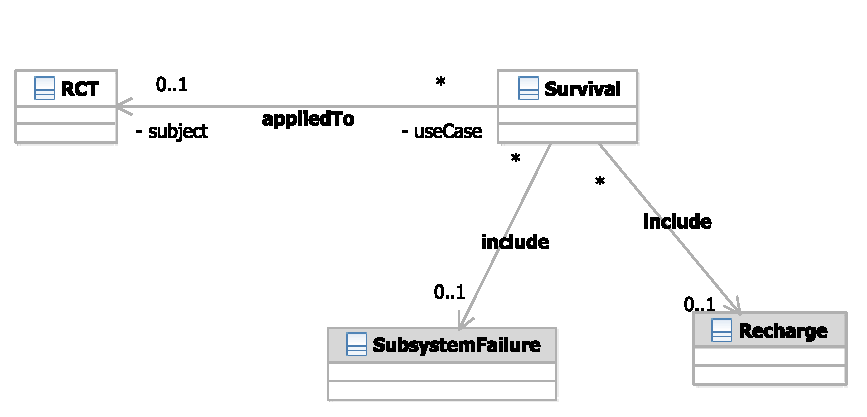
\includegraphics[width=0.85\textwidth]{RCT_RCTSurvivalUseCaseModel.pdf}}
\end{center}
\caption{RCT Survival UseCaseModel}
\label{survivalusecasemodel}
\end{figure}

It might be interesting to detail a particular \emph{UseCase} by paying attention to the \emph{Subsystem}s in the \emph{System}, to detail further \emph{Requirement}s. \emph{Subsystem}s identified in the RCT are the BasePlatform, the OnboardSystem, and the SupportingSystem. Focusing, for example, on the Navigation \emph{UseCase} previously defined, it is possible to identify additional \emph{Requirement}s for the \emph{Subsystem}s, in the form of a RCT Subsystem \emph{UseCaseModel} (Fig. \ref{rctnavigationsubsystemusecasemodel}).\\

\begin{figure}[htbp]
\begin{center}
 {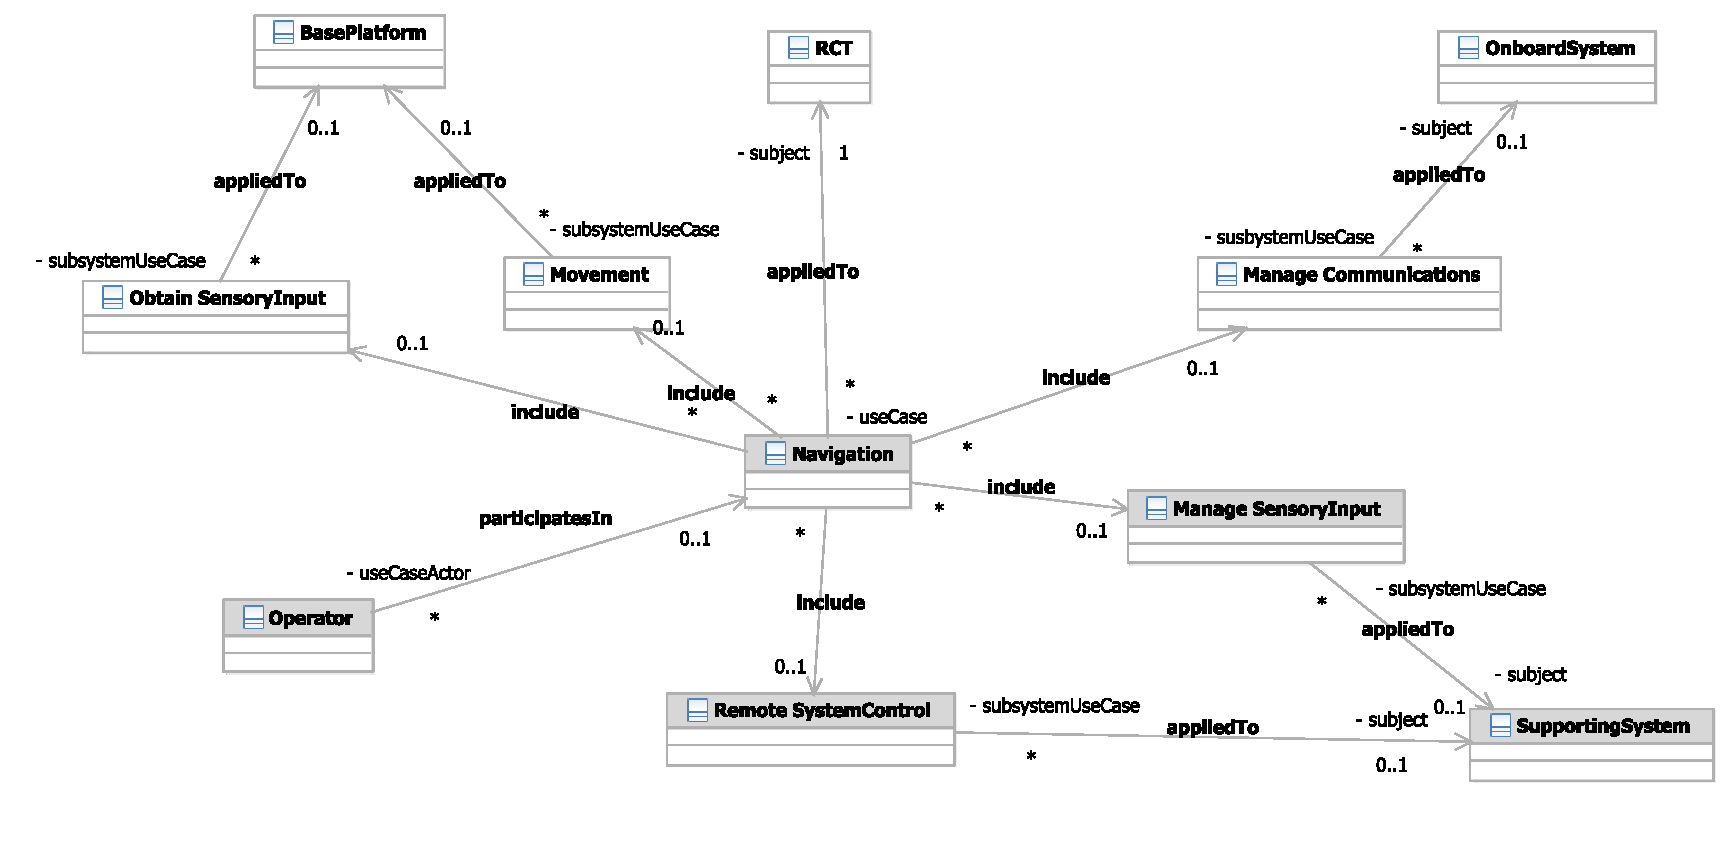
\includegraphics[width=0.95\textwidth]{RCT_SubsystemNavigationUseCaseModel.pdf}}
\end{center}
\caption{RCT Navigation UseCaseModel detailed for Subsystems}
\label{rctnavigationsubsystemusecasemodel}
\end{figure}

The \emph{UseCase Modelling Subtask} can also obtain a \emph{Subsystem UseCaseModel}, which gathers the \emph{Requirement} for a particular \emph{Subsystem}. In the case of the RCT, this subsystem usecasemodel was obtained for the BasePlatform (Fig. \ref{baseplatformusecasemodel}
 showing the instantiation of the original ontological elements) to detail the \emph{FunctionalRequirement} of movement; for the OnboardSystem to specify the \emph{FunctionalRequirement} of ManageCommunications (Fig. \ref{onboardusecasemodel}
); and for the SupportingSystem to clarify the Manage SensoryInput requirement (Fig. \ref{supportingsystemusecasemodel}).\\

\begin{figure}[htbp]
\begin{center}
 {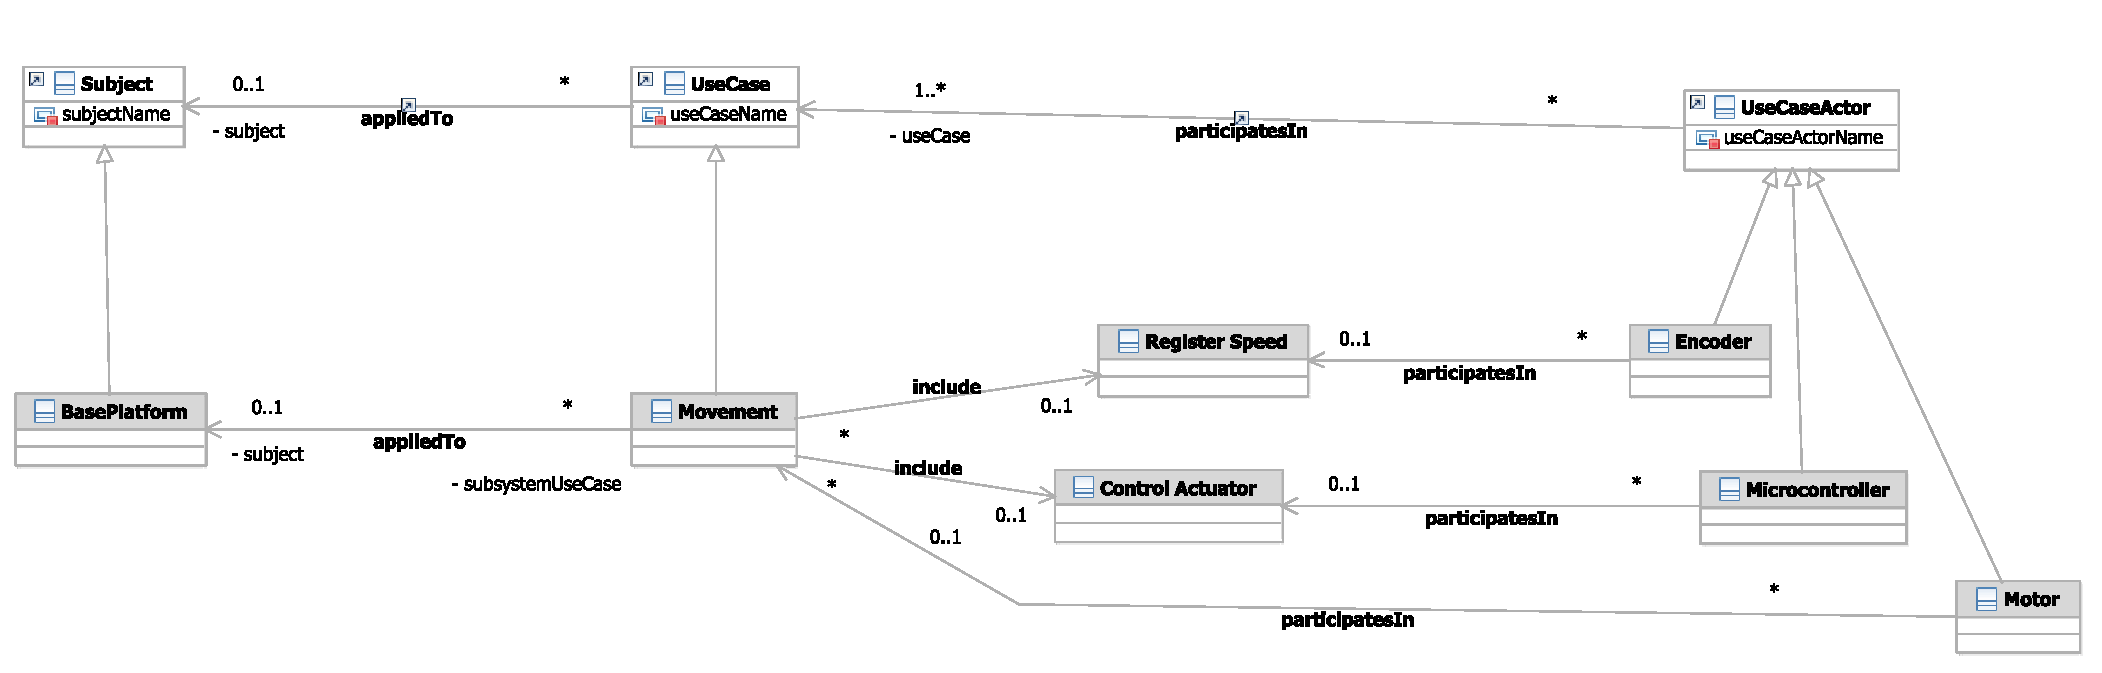
\includegraphics[width=0.85\textwidth]{RCT_BasePlatformMovementUseCaseModel.pdf}}
\end{center}
\caption{BasePlatform Subsystem UseCaseModel}
\label{baseplatformusecasemodel}
\end{figure}

\begin{figure}[htbp]
\begin{center}
 {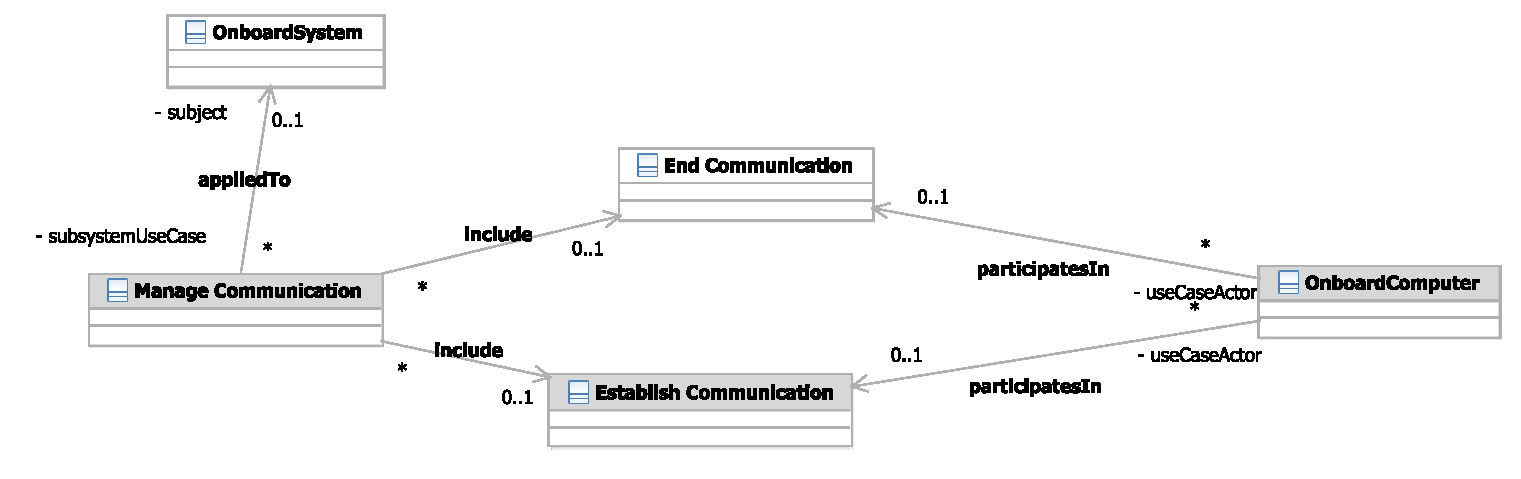
\includegraphics[width=0.85\textwidth]{RCT_OnBoardSystemManageCommunicationsUseCaseModel.pdf}}
\end{center}
\caption{OnboardSystem Subsystem UseCaseModel}
\label{onboardusecasemodel}
\end{figure}

\begin{figure}[htbp]
\begin{center}
 {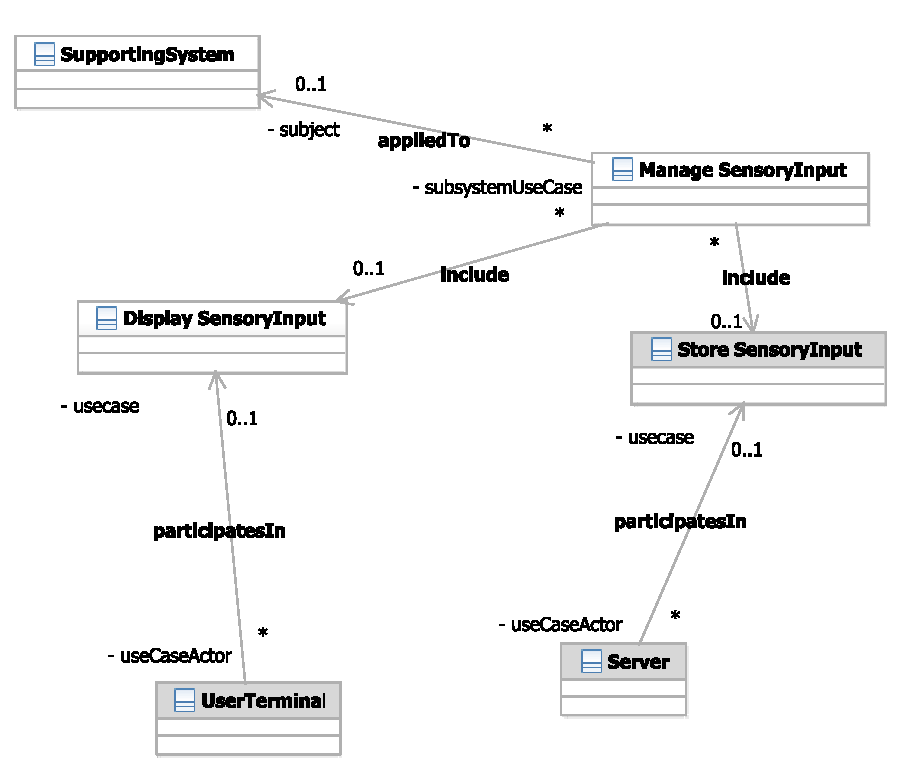
\includegraphics[width=0.75\textwidth]{RCT_SupportingSystemManageSensoryInputUseCaseModel.pdf}}
\end{center}
\caption{SupportingSystem Subsystem UseCaseModel}
\label{supportingsystemusecasemodel}
\end{figure}

The next \emph{Subtask} in the \emph{ASysRequirement Phase} is to detail each \emph{UseCaseModel} obtained during a \emph{UseCase Detailing Subtask}. This detail can be achieved by filling a pre--defined ASLab UseCase Pattern, with the relevant information in each field as required. This \emph{Subtask} was performed by the RCT developers, having as results different textual tables for the previous \emph{UseCase}s. For example, the detail for the Navigation requirement is shown in Fig. \ref{RCTnavigationdetailing}, and the Survival one in Fig. \ref{RCTsurvivaldetailing}.\\

\begin{figure}[htbp]
\begin{center}
 {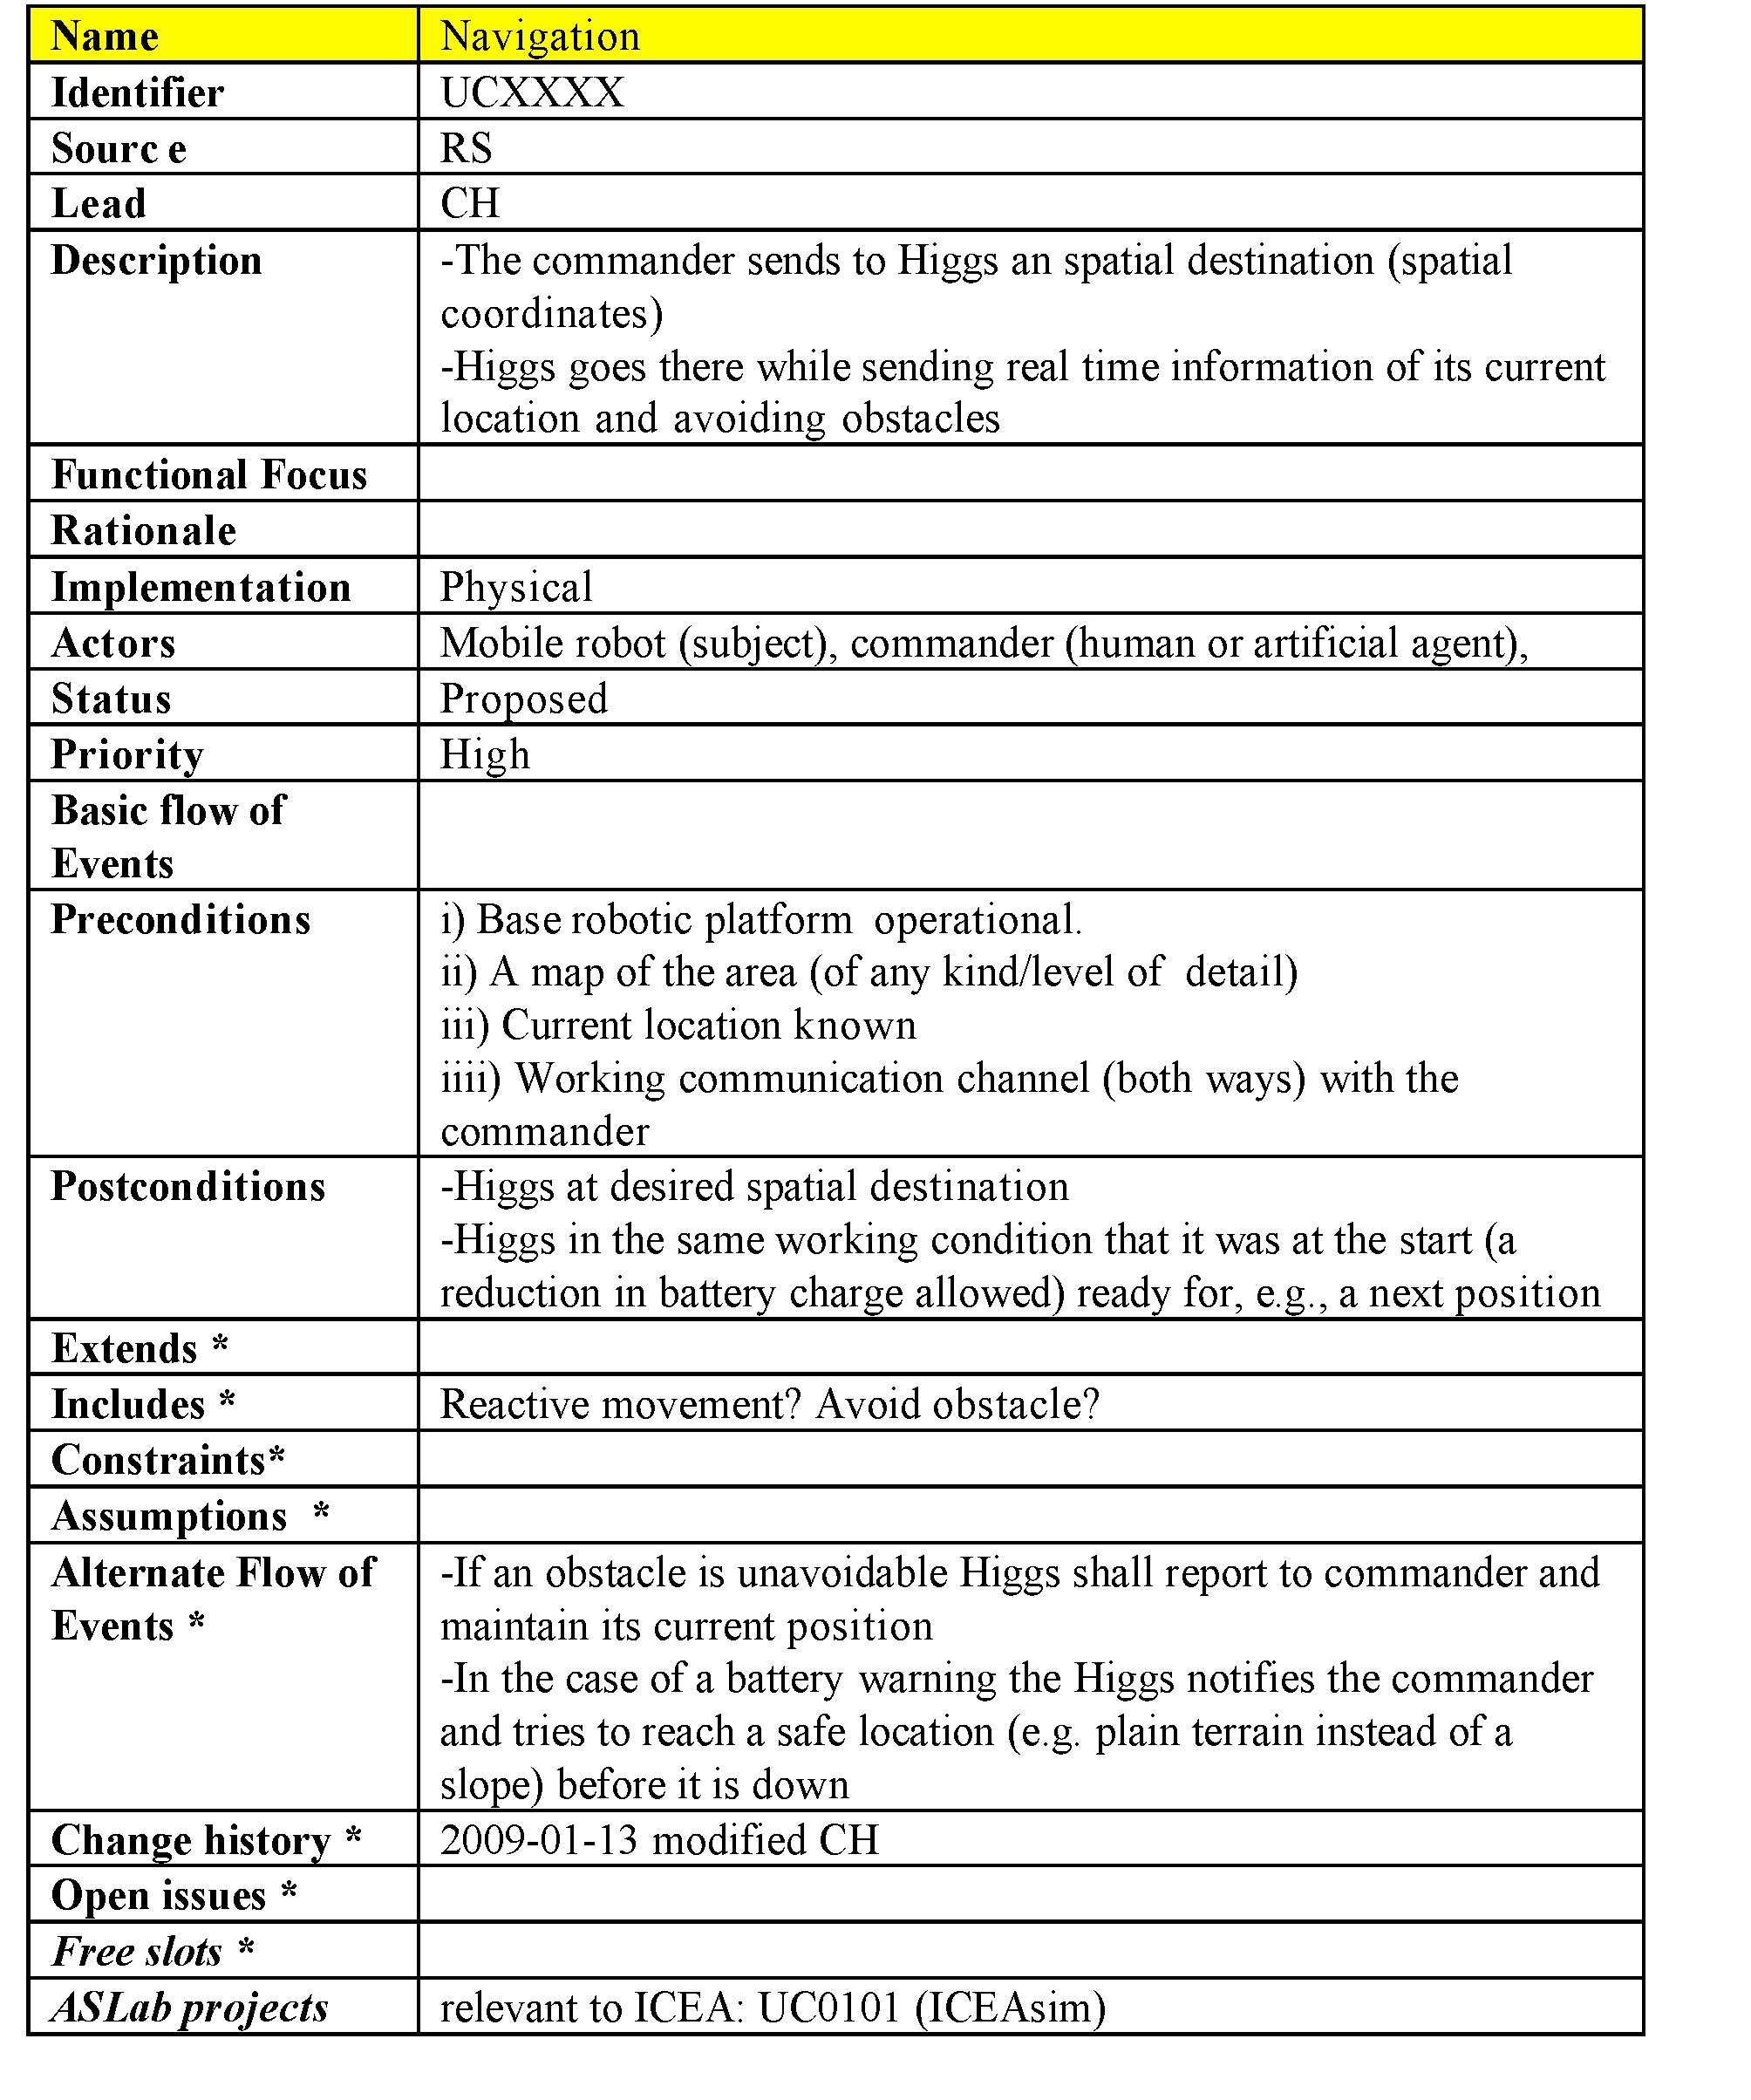
\includegraphics[width=0.75\textwidth]{RCT-NavigationUseCaseDetailing.pdf}}
\end{center}
\caption{UseCase Detailing Subtask for the Navigation requirement}
\label{RCTnavigationdetailing}
\end{figure}

\begin{figure}[htbp]
\begin{center}
 {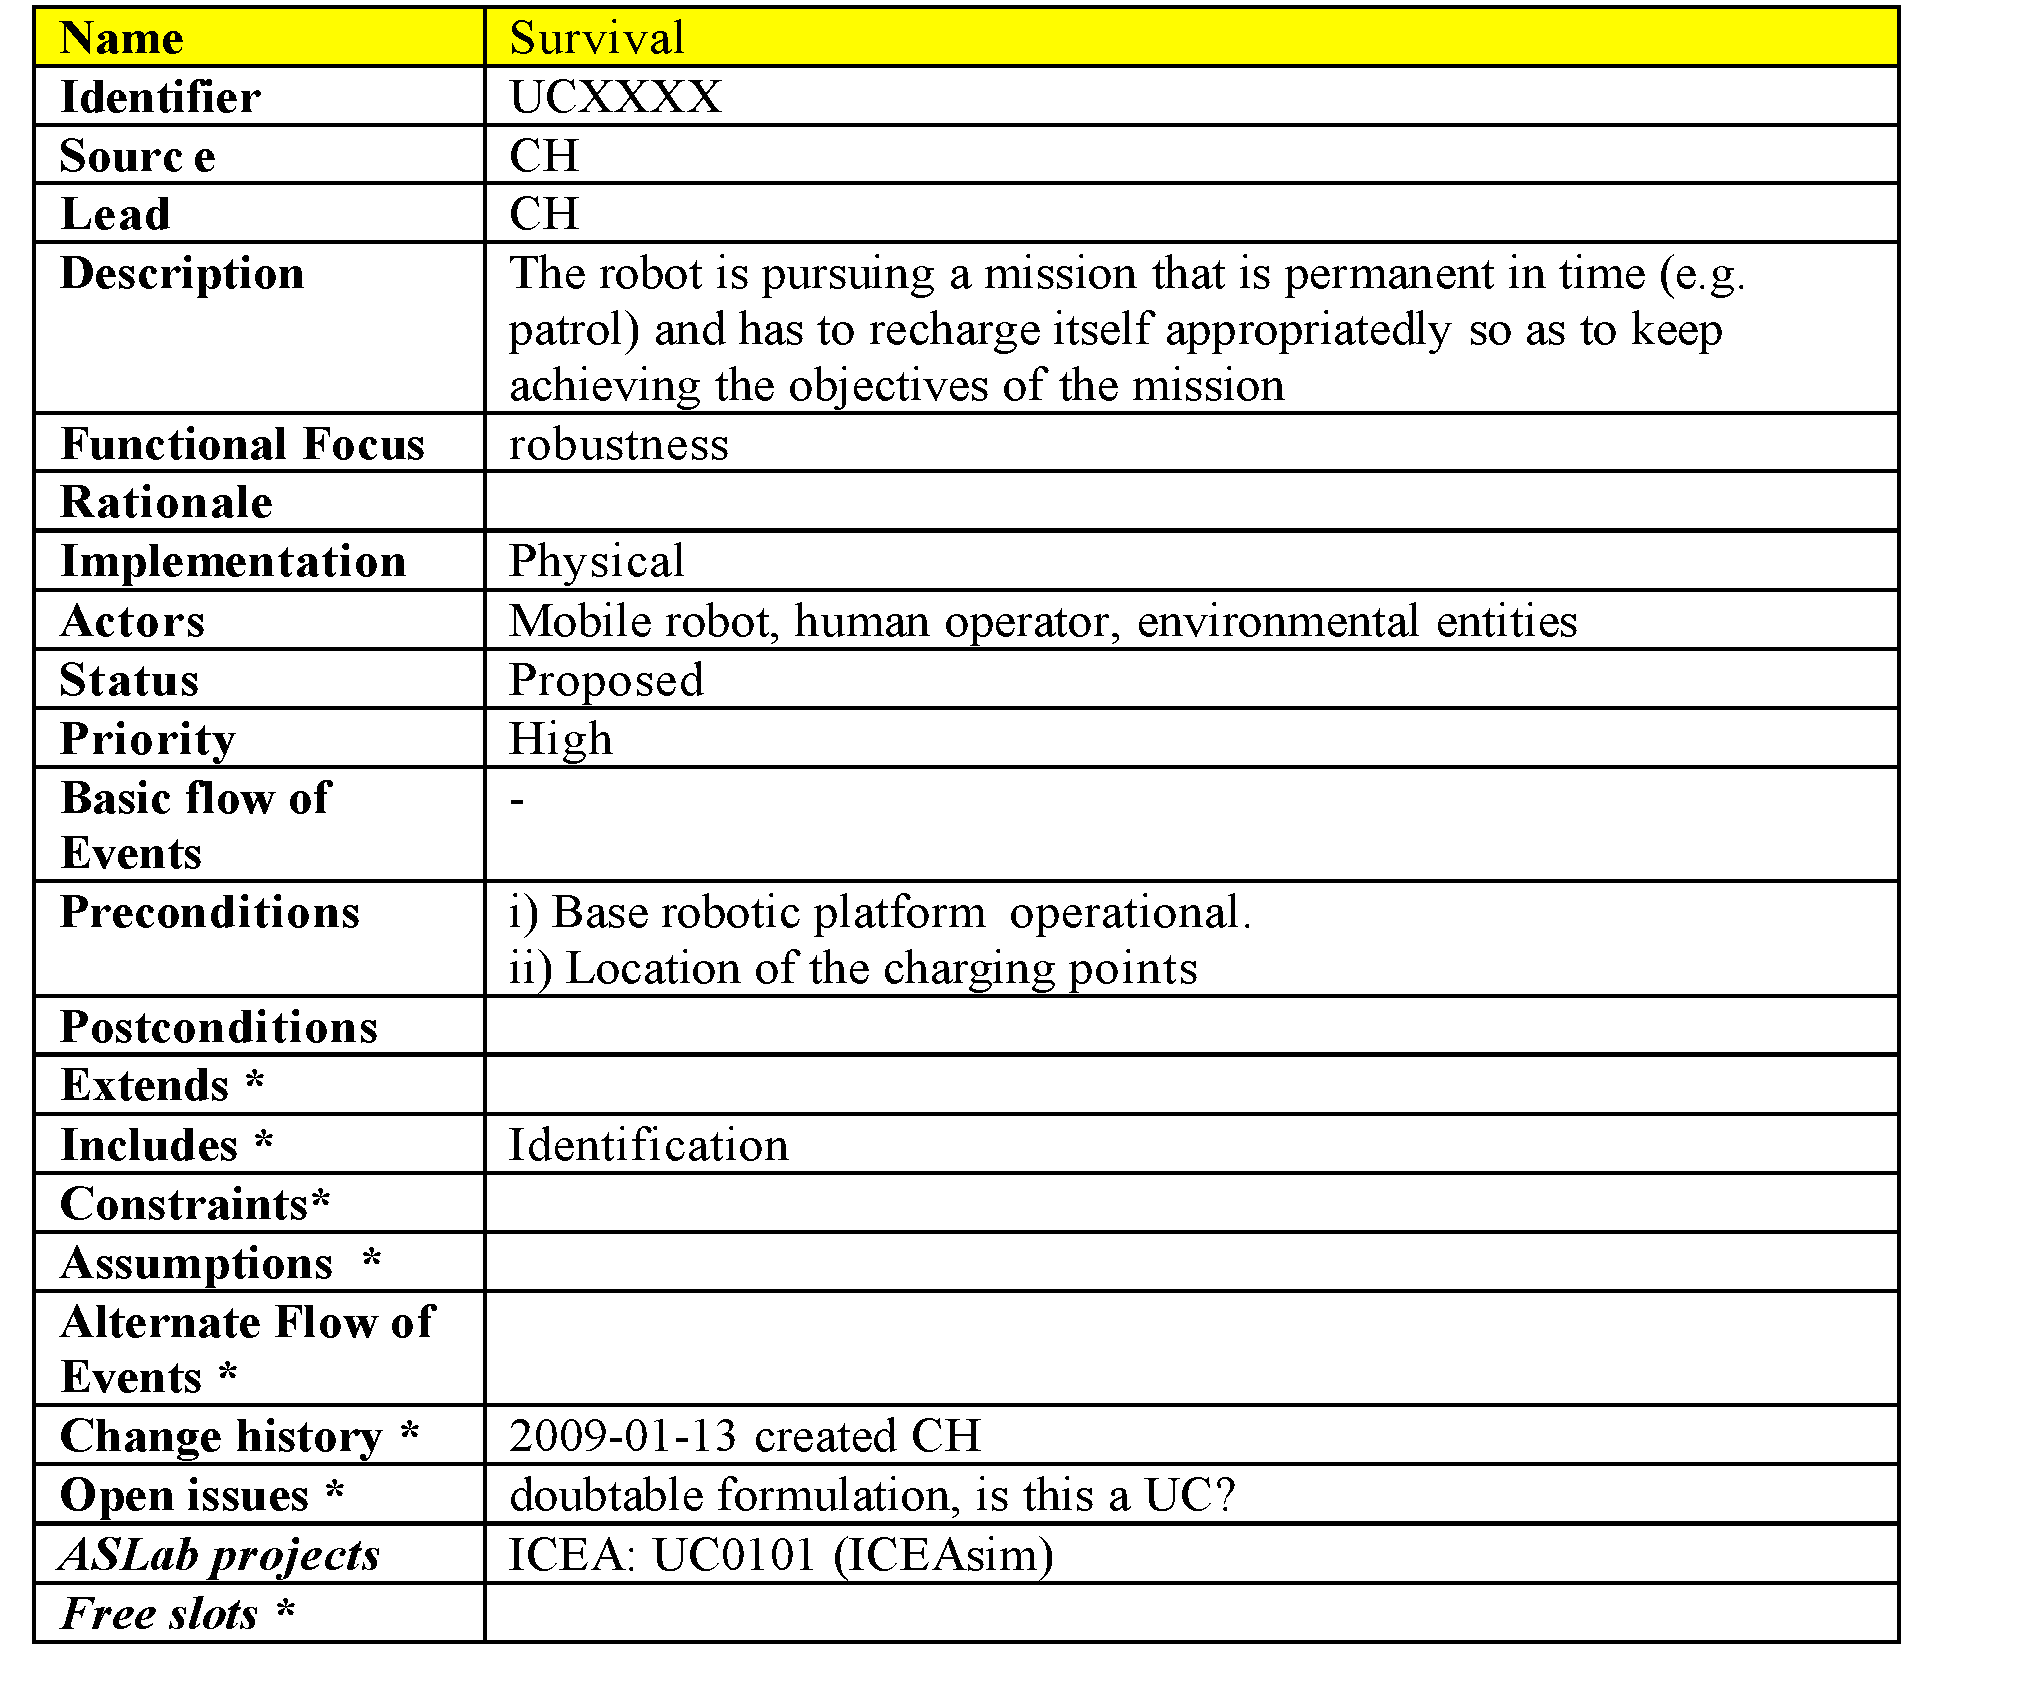
\includegraphics[width=0.75\textwidth]{RCT-SurvivalUseCaseDetailing.pdf}}
\end{center}
\caption{UseCase Detailing Subtask for the Survival requirement}
\label{RCTsurvivaldetailing}
\end{figure}


\item{Requirement Characterisation}

An additional \emph{Task} in this \emph{Phase} is to characterise the autonomous system's requirements, to obtain a \emph{RequirementCharacterisation}, as defined in the  ASys Engineering Process Package of the ASys Engineering Subontology. The taxonomies of concepts considered in the ASys Requirement Package can be described specifying a condition, a requirement criterion and a possible threshold. As a result, a \emph{Process Characterisation} and a \emph{System Characterisation} in the form of a textual description.\\ %look at MFESA book pp 374-375 to do this
\end{itemize}

\section{RCT ASys Analysis Phase}

As part of the ASys Analysis Phase consists of differents \emph{Tasks}, such as \emph{StructuralAnalysis}, \emph{BehaviouralAnalysis}, and \emph{FunctionalAnalysis}. The differents tasks have been carried out for the Robot Control Testbed, as described in following sections.\\

\begin{description}
\item \textbf{Structural Analysis}\\

The \emph{StructuralAnalysis Task} pays attention to the system under analysis from a \emph{StructuralViewpoint}, i.e., the analysis considering the system's structure in terms of subsystems and elements. As outcome of the task, a \emph{StructuralModel} for the RCT is obtained, consisting of \emph{StructureModel}s and\emph{Topology Model}s.\\

\begin{itemize}
\item System Modelling\\

The \emph{SystemModelling Subtask} carried out for the RCT has obtained the \emph{StructuralModel}, consisting of the \emph{StructureModel}s and the \emph{TopologyModel}s. For the RCT \emph{StructureModel}, the different subsystems part of it were determined according to the structural definition provided. Hence, three different kind of subsystem were identified: the platform, the onboard system attached to it, and the supporting system which are not physically part of the RCT but take part into its operation. The platform was further analysed to identify the subsystems or elements part of it. The different onboard systems were identified. Finally, the supporting systems were specified. The overall analysis result was formalised as a \emph{StructureModel} for the RCT (Fig. \ref{fig:RCTsystemmodel}). \\

\begin{figure}[htbp]
\begin{center}
 {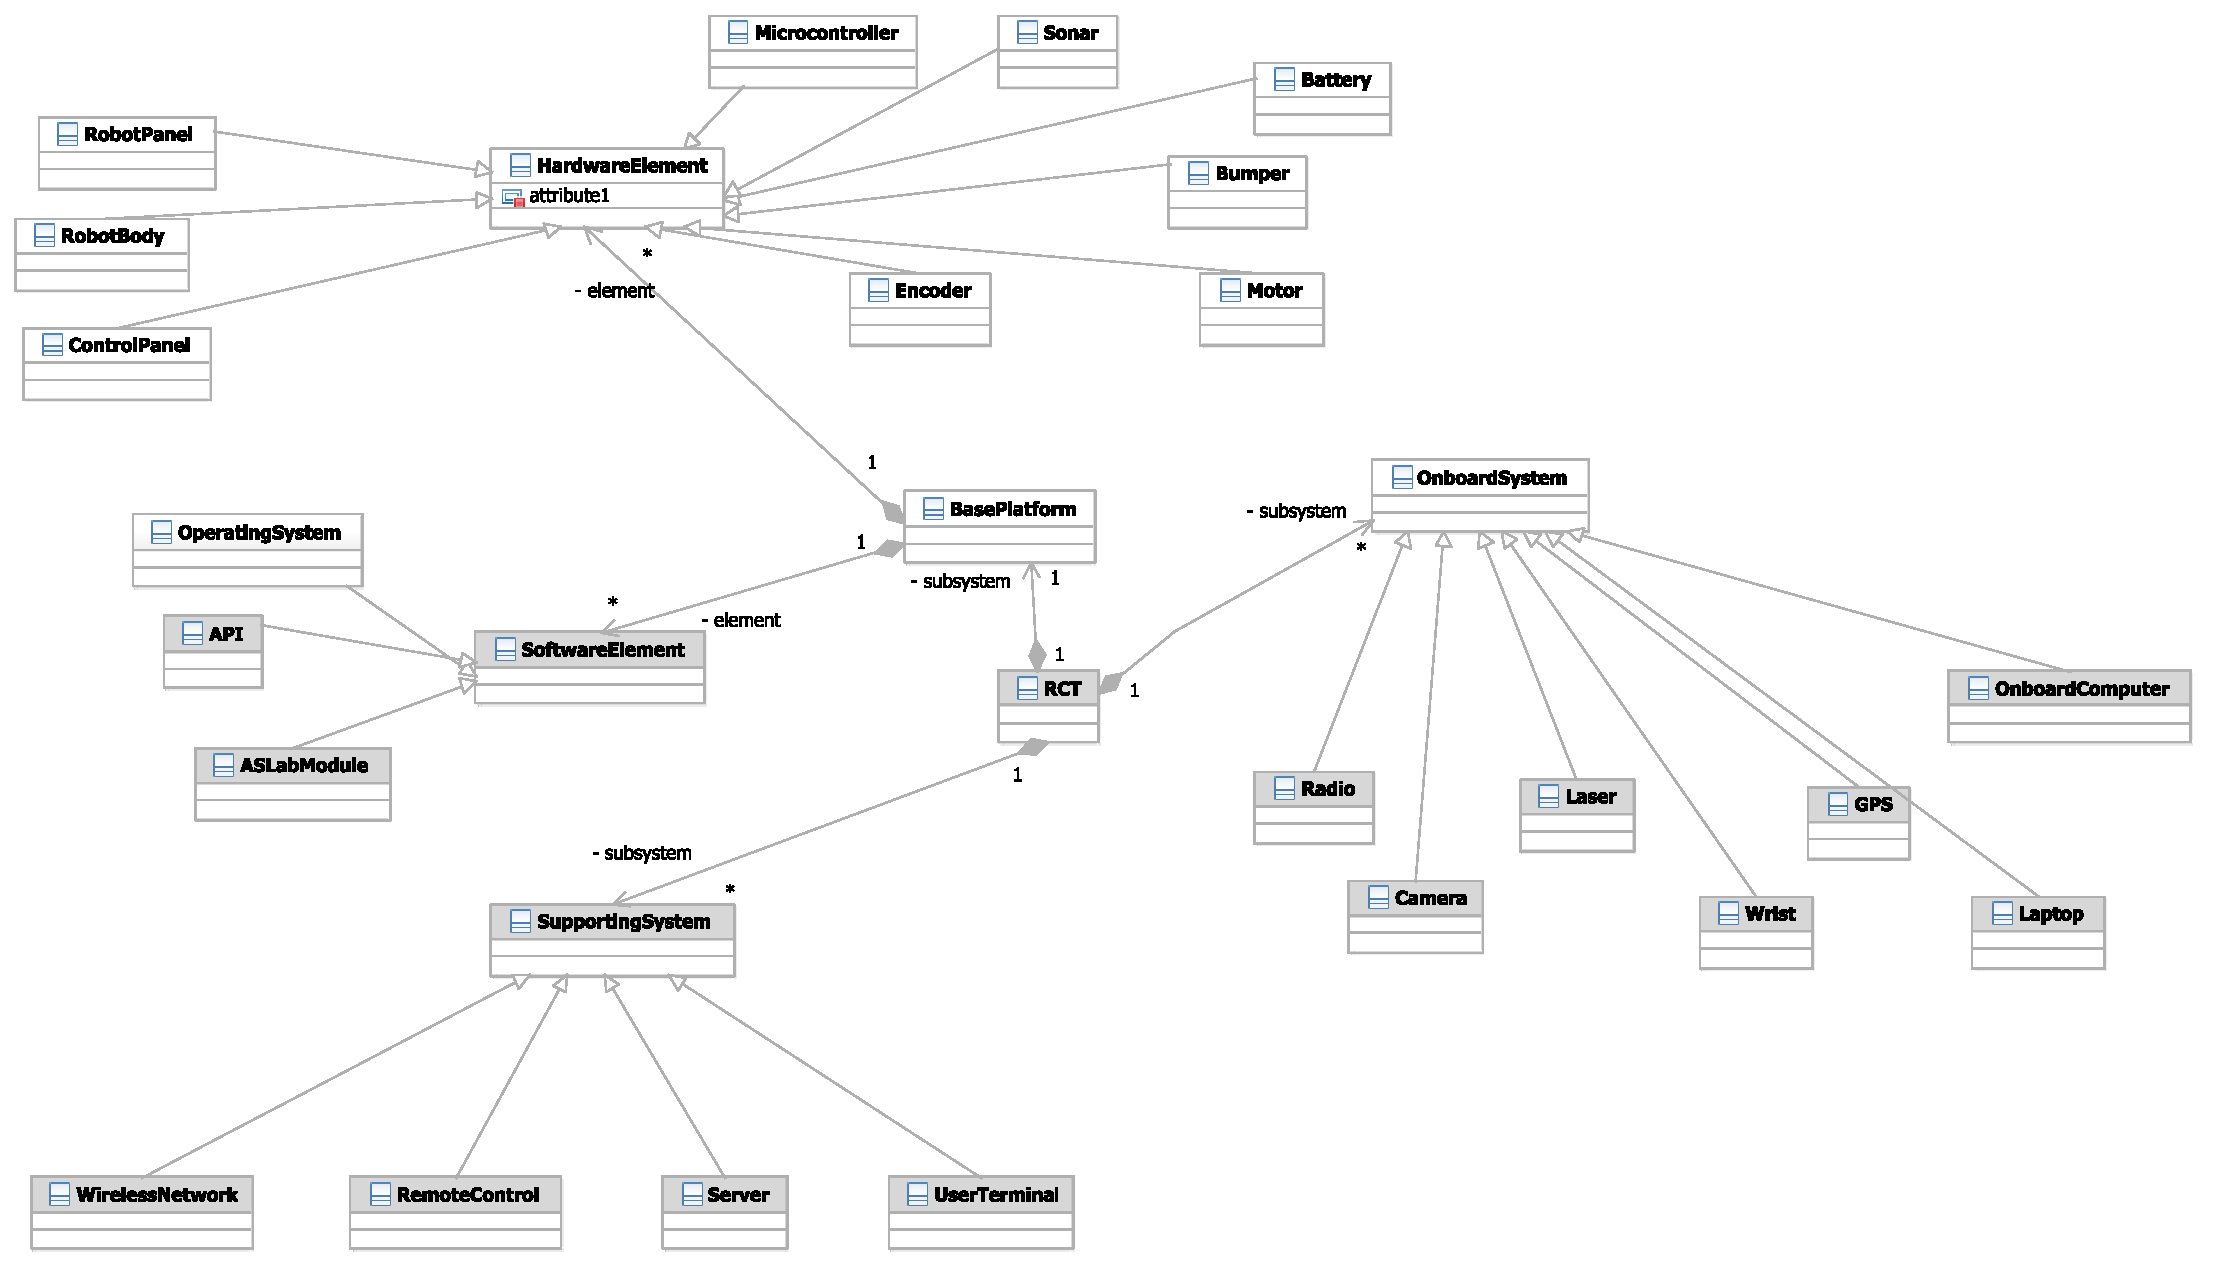
\includegraphics[width=0.99\textwidth]{RCT_RCTStructureModel_1.pdf}}
\end{center}
\caption{RCT Structure Model}
\label{fig:RCTsystemmodel}
\end{figure}


The \emph{TopologyModel} allows representing the topological connections between a system's parts, by refining the Topology Package concepts. For the Robot Control Testbed, it was considered important to differentiate the topology from an informational and a physical aspects. The first one refers to the communication connections between parts, such as WiFi, Ethernet, etc. The latter, the physical connections among parts in a traditional way. Hence, two different topology models have been obtained for the RCT system: the RCT Informational Topology Model (Fig. \ref{fig:RCTinformationaltopologymodel}), and the RCT Physical Topology Model (Fig. \ref{fig:RCTphysicaltopologymodel}).\\

\begin{figure}[htbp]
\begin{center}
 {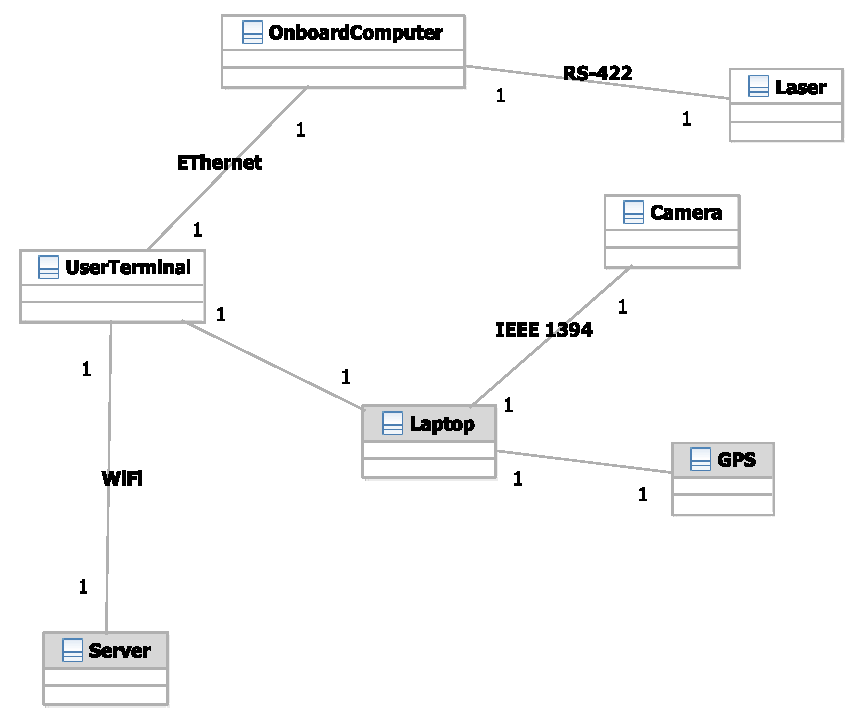
\includegraphics[width=0.75\textwidth]{RCT_RCTInformationalTopologyModel.pdf}}
\end{center}
\caption{RCT Topology Model: informational connections}
\label{fig:RCTinformationaltopologymodel}
\end{figure}

\begin{figure}[htbp]
\begin{center}
 {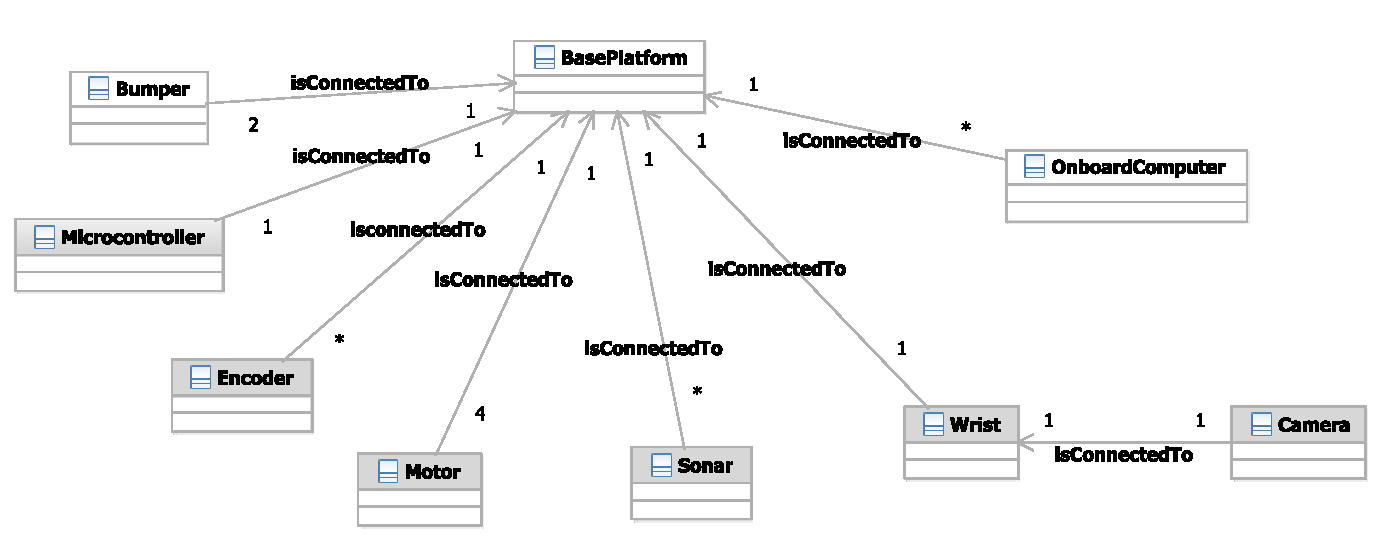
\includegraphics[width=0.99\textwidth]{RCT_RCTPhysicalTopologyModel.pdf}}
\end{center}
\caption{RCT Topology Model: physical connections}
\label{fig:RCTphysicaltopologymodel}
\end{figure}

Each one of the subsystems and elements identified in the \emph{StructureModel}, can be further detailed during a design phase to represent their characteristics and roles, by ontologically instantiating the concepts in the PhysicalDevice Package into a \emph{DeviceModel}. \\

%23 March 2010: I cannot longer use this, as I do not know how to make for the RSA does not show the values for the attributes
%An example is given in Fig. \ref{fig:RCTdevicemodel} for the Base Platform of the Robot Control Testbed. Additional attributes have been added as required, e.g. in the PowerSupply concept, to express specific design elements not included in the general ontological element. In a similar way, the computational devices and components can be detailed considering the Computational Device Package, to express software components, devices, and interfaces.\\

%\begin{figure}[htbp]
%\begin{center}
% {\includegraphics[width=0.90\textwidth]{RCT-DeviceModel.pdf}}
%\end{center}
%\caption{RCT Base Platform Device Model during design phase}
%\label{fig:RCTdevicemodel}
%\end{figure}


%TBD\item Knowledge Modelling

\end{itemize}
%TBD\item \textbf{Behavioural Analysis}

%TBD\item \textbf{Functional Analysis}

\end{description}

